\def\duedate{12/18/22}
\def\HWnum{Final}
% Document setup
\documentclass[12pt]{article}
\usepackage[margin=1in]{geometry}
\usepackage{fancyhdr}
\usepackage{lastpage}

\pagestyle{fancy}
\lhead{Richard Whitehill}
\chead{PHYS 675 -- HW \HWnum}
\rhead{\duedate}
\cfoot{\thepage \hspace{1pt} of \pageref{LastPage}}

% Encoding
\usepackage[utf8]{inputenc}
\usepackage[T1]{fontenc}

% Math/Physics Packages
\usepackage{amsmath}
\usepackage{mathtools}
\usepackage[arrowdel]{physics}
\usepackage{siunitx}

\AtBeginDocument{\RenewCommandCopy\qty\SI}

% Reference Style
\usepackage{hyperref}
\hypersetup{
    colorlinks=true,
    linkcolor=blue,
    filecolor=magenta,
    urlcolor=cyan,
    citecolor=green
}

\newcommand{\eref}[1]{Eq.~(\ref{eq:#1})}
\newcommand{\erefs}[2]{Eqs.~(\ref{eq:#1})--(\ref{eq:#2})}

\newcommand{\fref}[1]{Fig.~\ref{fig:#1}}
\newcommand{\frefs}[2]{Figs.~\ref{fig:#1}--\ref{fig:#2}}

\newcommand{\tref}[1]{Table~\ref{tab:#1}}
\newcommand{\trefs}[2]{Tables~\ref{tab:#1}-\ref{tab:#2}}

% Figures and Tables 
\usepackage{graphicx}
\usepackage{float}
\usepackage{booktabs}

\newcommand{\bef}{\begin{figure}[h!]\begin{center}}
\newcommand{\eef}{\end{center}\end{figure}}

\newcommand{\bet}{\begin{table}[h!]\begin{center}}
\newcommand{\eet}{\end{center}\end{table}}

% tikz
\usepackage{tikz}
\usetikzlibrary{calc}
\usetikzlibrary{decorations.pathmorphing}
\usetikzlibrary{decorations.markings}
\usetikzlibrary{arrows.meta}
\usetikzlibrary{positioning}

% tcolorbox
\usepackage[most]{tcolorbox}
\usepackage{xcolor}
\usepackage{xifthen}
\usepackage{parskip}

\newcommand*{\eqbox}{\tcboxmath[
    enhanced,
    colback=black!10!white,
    colframe=black,
    sharp corners,
    size=fbox,
    boxsep=8pt,
    boxrule=1pt
]}

% Miscellaneous Definitions/Settings
\newcommand{\prob}[2]{\textbf{#1)} #2}

\setlength{\parskip}{\baselineskip}
\setlength{\parindent}{0pt}
\setlength{\headheight}{14.49998pt}
\addtolength{\topmargin}{-2.49998pt}

\usepackage[]{amssymb}

\begin{document}
    
\prob{3}{
What is the lowest kinetic energy for a proton to produce Cherenkov radiation in water?
}

The speed of light in a medium with index of refraction $n$ is $c_{m} = c/n$, and Cherenkov radiation is produced when the speed of a particle in this medium is greater than the speed of light in the same medium: $v > c_{m}$.
Equivalently, we require $v/c = \beta > 1/n$.
The kinetic energy of a relativistic particle with speed $v$ is
\begin{eqnarray}
    T = (\gamma - 1)mc^2 = \Big( \frac{1}{\sqrt{1 - \beta^2}} - 1 \Big) mc^2
.\end{eqnarray}
Solving this expression for $\beta$ we find
\begin{eqnarray}
    \beta^2 = 1 - \frac{1}{\Big( 1 + \frac{T}{mc^2} \Big)^2} > \frac{1}{n^2}
\end{eqnarray}
for the production of Cherenkov radiation.
Rearranging to give a requirement for the threshold value of $T$, we obtain
\begin{eqnarray}
    T > \Big( \Big[ 1 - \frac{1}{n^2} \Big]^{-1/2} - 1 \Big) mc^2
.\end{eqnarray}
For a proton ($m = \SI{0.938}{\GeV/c^2}$)we find that the threshold kinetic energy for the production of Cherenkov radiation in water ($n = 1.333$) is
\begin{eqnarray}
    T_{\rm min} = \SI{0.481}{\GeV}
.\end{eqnarray}

\prob{4}{
At what energy scales is QCD predicted to become perturbative?
Do experimental observation back this up?
Briefly describe what evidence exists.
}

The following plot is given in \href{https://arxiv.org/pdf/1604.08082.pdf}{this paper}:
\begin{center}
    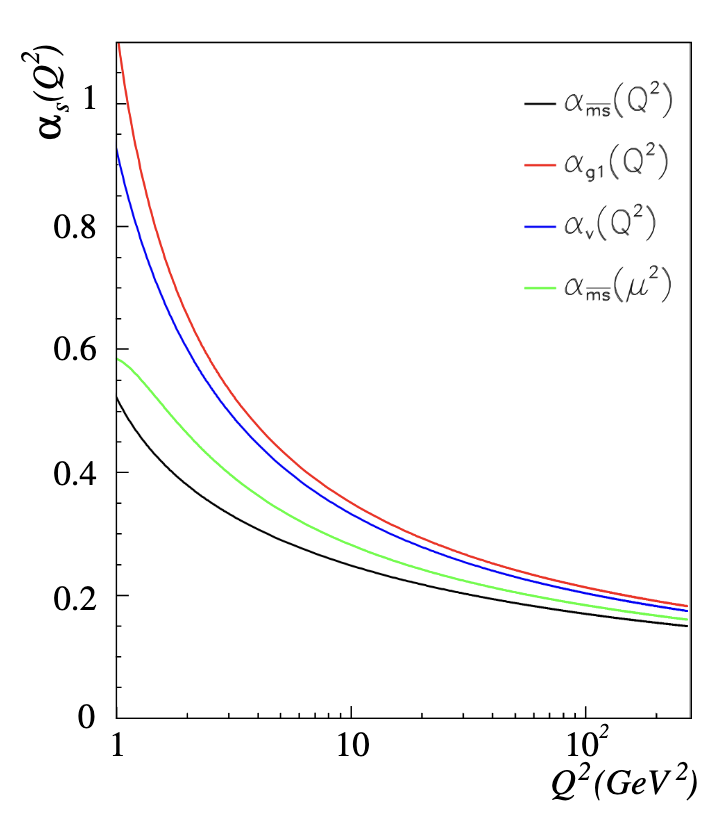
\includegraphics[width=0.4\textwidth]{prob4.png}
\end{center}
In different schemes, $\alpha_{s}$ has different behavior.
The most conventional choice in the literature is the $\overline{MS}$ renormalization scheme, which is the black line.
From this, we can see that QCD is perturbative for $Q^2 \gtrsim \SI{2}{\GeV^2}$.
In perturbative calcualtions in QCD, it is conventional to set the lower limit of the perturbative scale at the mass of the charm quark (i.e. $Q^2 \gtrsim m_{c}^2 = (\SI{1.275}{\GeV})^2$.

Experimental results give good agreement with applications of perturbation theory in processes such as DIS, which has had much success with the determination of $\alpha_{s}$ at the mass of the $Z$ boson using the Bjorken and Gross-Llewellyn Smith sum rules for $Q^2 > \SI{1}{\GeV^2}$.
Incorporating allall  world data, the value for the strong coupling $\alpha_s(M_{Z}^2) = 0.1123 \pm 0.0061$, which is a very precise value.
Additionally, the jet production process in DIS has been successful in determining $\alpha_{s}$ and in demonstrating the compatibility of perturbative calculations to the experimental results.

\prob{5}{
What is a glueball?
Describe with the ideas from QCD we discussed this semester.
Have glueballs been observed?
Discuss.
}

Glueballs are composite bound states predicted by QCD with no valence quarks.
That is, they are made of gluons and sea quarks.
Essentially, glueballs can be imagined to be particles made up of gluons interacting with each other, which can also create $q\bar{q}$ pairs from the vacuum but eventually annihilate.
The current theoretical work postulates that glueballs exist in energy scales which are accessible to our modern colliders, but they have not been observed because of several complications.
One of the significant complication is that glueballs mix with other meson states, which complicates the identification of glueballs compared with particles that exist as pure states.
At present there are multiple candidate particles that have been observed in experiments, but none match the expected properties of a glueball to enough precision such that we can confirm the existence of glueballs, but there are a few active experimental collaborations whose objective is to produce more definitive evidence for the existence of glueballs.

\prob{6}{
What observation did the EMC make that led to the proton spin crisis?
}

Since the proton has a $uud$ valence, it is expected that most of the proton spin, which is naively assumed to be in its S-wave state, comes from the $u$ and $d$ quarks.
Using these assumptions and sprinkling in some QCD corrections, we can derive a sum rule for the $g_{1}$ polarized structure function which is predicted in this model to have a value
\begin{eqnarray}
    \int_{0}^{1} \dd{x} g_{1}(x,Q^2=\SI{10}{\GeV^2}) = 0.171 \pm 0.006
.\end{eqnarray}
This integral is related to $\Delta \Sigma = \sum_{i} \Delta q_{i}$, which is interpreted as the spin contribution from the quarks and antiquarks to the proton.
The EMC experiment measured the double longitudinal spin asymmetry in polarized DIS and determined the $g_1$ structure function from its relationship to these measurements.
By integrating $g_1$, the EMC experimental collaboration was able to extract a value $\Delta \Sigma = 0.14 \pm 0.18$, which has a much smaller nominal value than expected.
In the parton model that Ellis and Jaffe used to derive their result, it was derived that $\Delta \Sigma \sim 1$, as expected intuitively.
This result implied that the quark spin contributed very little to the overall proton spin, meaning that gluon spin and orbital angular momentum contributions are more significant than anticipated.
Additionally, the EMC measurement implied that the strange sea was significantly polarized, which is surprising.

\prob{7}{
Show explicitly that the CKM matrix is unitary using the following parameterization
\begin{eqnarray}
    V_{CKM} = \begin{pmatrix}
        c_{12}c_{13} & s_{12}c_{13} & s_{13}e^{-i\delta} \\
        -s_{12}c_{23} - c_{12}s_{23}s_{13}e^{i\delta} & c_{12}c_{23} - s_{12}s_{23}s_{13}e^{i\delta} & s_{23}c_{13} \\
        s_{12}s_{23} - c_{12}c_{23}s_{13}e^{i\delta} & -c_{12}s_{23} - s_{12}c_{23}s_{13}e^{i\delta} & c_{23}c_{13}
    \end{pmatrix}
,\end{eqnarray}
where $c_{ij} = \cos{\theta_{ij}}$, $s_{ij} = \sin{\theta_{ij}}$, and $\delta \in \real$.
}

The work was done by the \textit{sympy} package in python, and because the computations are quite cumbersome, the work is shown in the screenshot below:
\begin{center}
    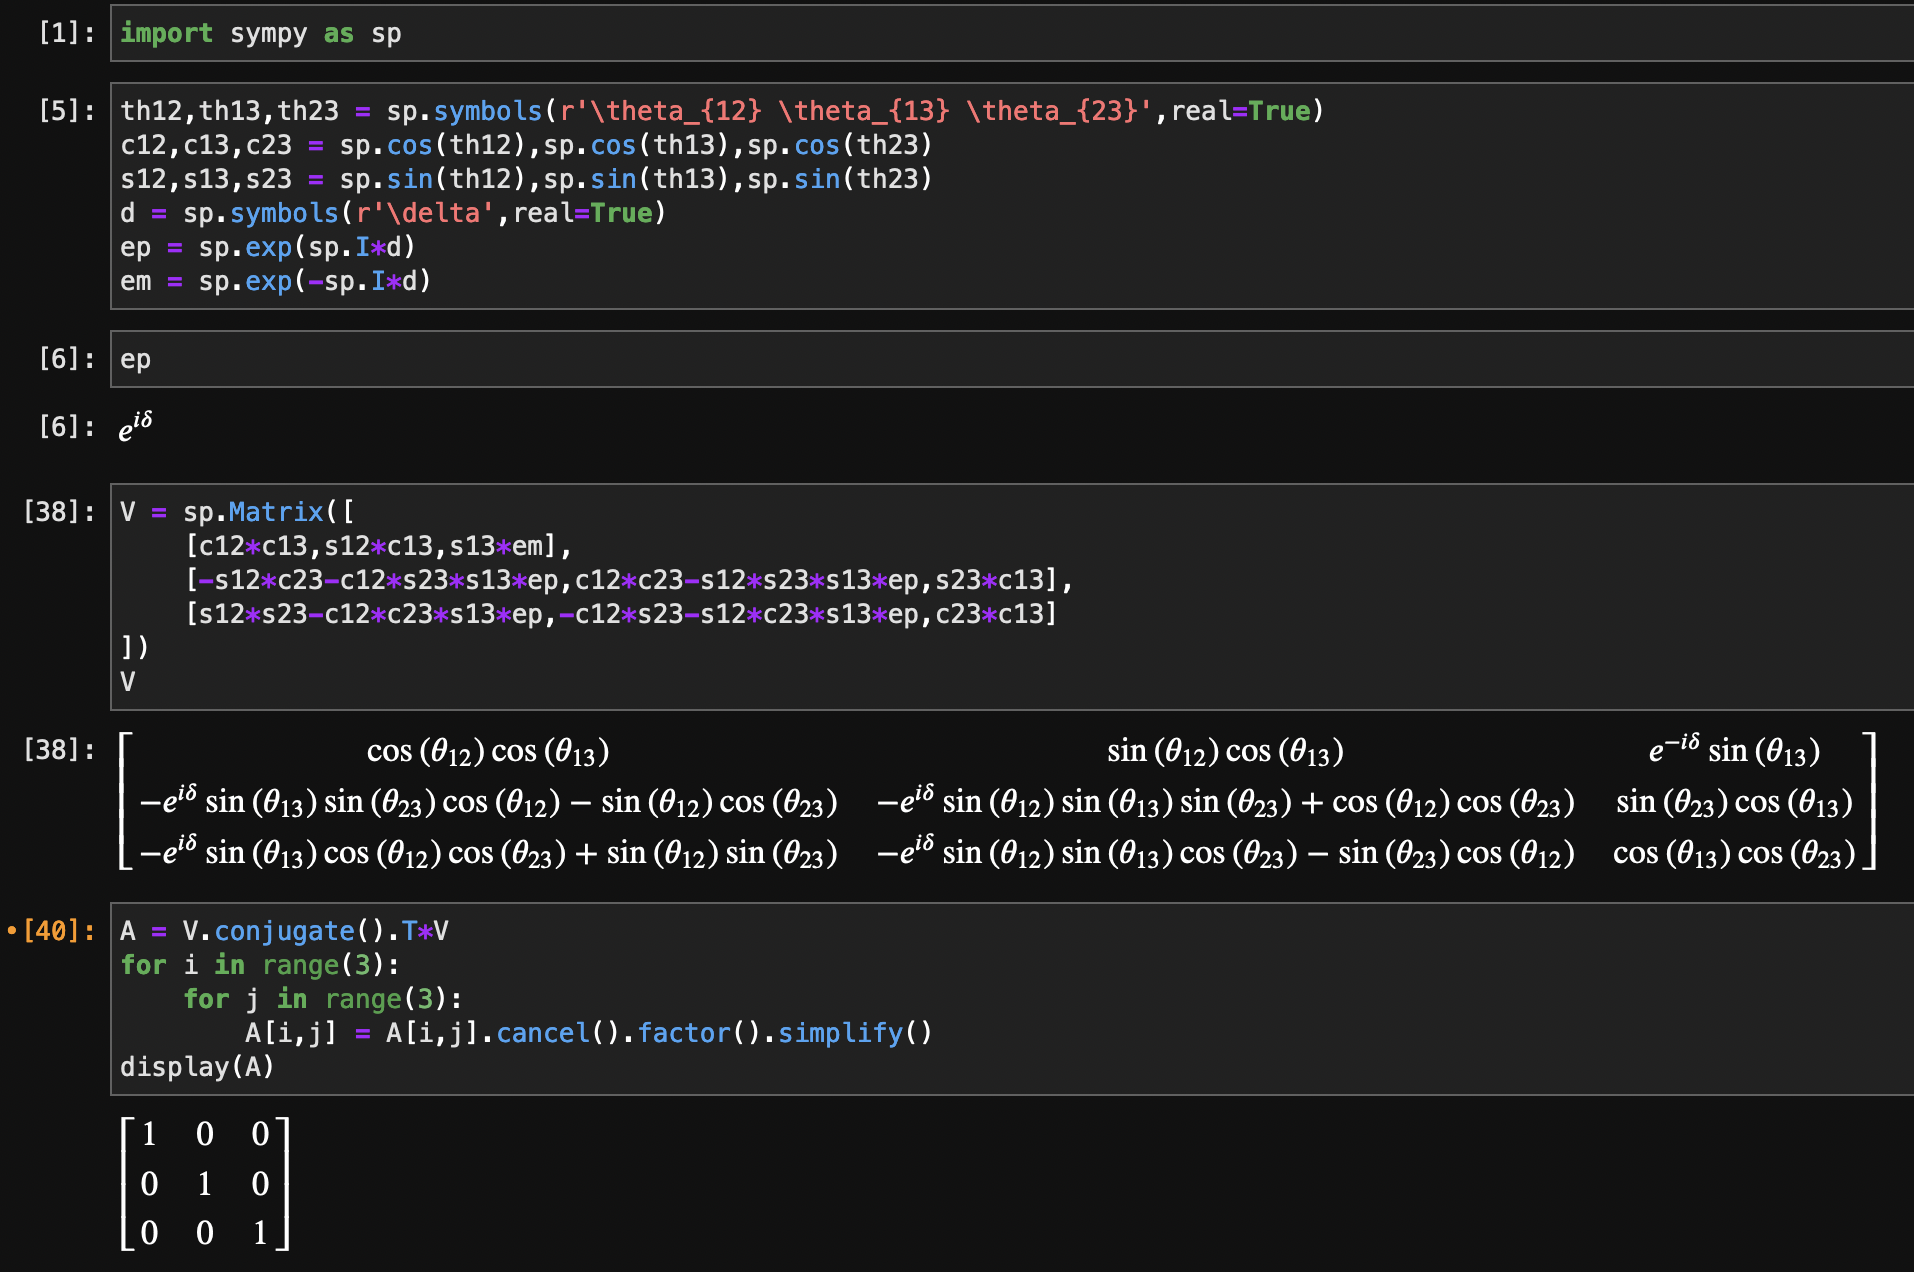
\includegraphics[width=\textwidth]{./prob7.png}
\end{center}
The result verifies that $V_{CKM}^{\dagger}V_{CKM} = 1$



\end{document}
